\chapter{Pipeline extraction} \label{chapter4}

\section{Introduction}


The previous chapter presented globally the state of the art in designing systems to scale in performance, and in maintenance.
It refined the scope of this thesis to the study of the opposition between maintenance scalability and performance scalability in streaming web applications.
It concluded with the objectives of this thesis, which is to find an equivalence between the two opposed organizations.
The maintenance scalability organization, supported by modular programming, higher-order programming and a global memory store.
The performance scalability organization, supported by the parallelism of memory and exuction distribution.
The equivalence between these two organization is in two steps, as presented in figure \ref{fig:chapter3:objectives:roadmap}.
This chapter presents the first step in this equivalence.
That is to identify and extract a pipeline of execution inside an application following the first organization.
In this work, we focus on Javascript, and specifically node.js applications.
In this chapter, I define further the higher-order programming concepts.

In Javascript, functions are first-class citizens ; it allows to manipulate them like any object, and to link them to react to asynchronous events, \textit{e.g.} user inputs and remote requests.
These asynchronously triggered functions are named callbacks, and allow to efficiently cope with the distributed and inherently asynchronous architecture of the Internet.
To execute a suite of asynchronous functions, callbacks are nested one into the other.
This nesting, if not organized properly, can result in unreadable layer of callbacks, commonly presented as \textit{callback hell}\ftnt{http://maxogden.github.io/callback-hell/}, or \textit{pyramid of doom}.

Promises are another way to organize a suite of asynchronous operations avoiding this callback hell.
They organize the operations as a well-defined pipeline.
Moreover, Promises provide additional control over the asynchronous execution flow, than callbacks.
They are part of the next version of the Javascript language, ECMAScript 6\ftnt{http://people.mozilla.org/~jorendorff/es6-draft.html}.
To avoid the equivalence being unnecessarily incomplete, we present an alternative to Promise, called Due.
Due organize the operations like Promises, as a well-defined pipeline, while discarding the unnecessary additional control over the asynchronous flow.

This chapter present an equivalence, and a compiler to identify the pipeline of operating underlying in a Javascript application using callbacks, and extract it to express it as Dues.
This compiler has been tested over 64 \textit{Node.js} packages from the node package manager (npm\ftnt{https://www.npmjs.com/}).
55 packages were incompatible with the compiler, 9 packages were compiled with success.

Callbacks, Promises and Dues are further defined in section \ref{section:definitions}.
Section \ref{section:equivalence} explains the transformation from imbrications of callbacks to sequences of Dues.
Section \ref{section:compiler} presents a compiler to automate the application of this equivalence.
And finally, the developed compiler is evaluated in section \ref{section:evaluation}.


% This made Javascript a language of choice to develop both client and, more recently, server applications for the web.

% Callbacks are well-suited for small interactive scripts.
% But in a complete application, they are ill-suited to control the larger asynchronous execution flow.
% Their use leads to intricate imbrications of function calls and callbacks, commonly presented as \textit{callback hell}\ftnt{http://maxogden.github.io/callback-hell/}, or \textit{pyramid of doom}.
% This is widely recognized as a bad practice and reflects the unsuitability of callbacks in complete applications.
% Eventually, developers enhanced callbacks to meet their needs with the concept of Promise~\cite{Liskov1988}.

% Promises bring a different way to control the asynchronous execution flow, better suited for large applications.
% They fulfill this task well enough to be part of the next version of the Javascript language, ECMAScript 6\ftnt{http://people.mozilla.org/~jorendorff/es6-draft.html}.
% However, because Javascript started as a scripting language, beginners are often not introduced to Promises early enough.
% Most APIs use the classical callback approach encouraging beginner in this practice.
% Moreover, despite its benefits, the concept of Promise is not yet widely acknowledged.
% Developers may implement their own library for asynchronous flow control before discovering existing ones.
% There is such a disparity between the needs for and the adoption of Promises libraries, that there are almost 40 different implementations\ftnt{https://github.com/promises-aplus/promises-spec/blob/master/implementations.md}.

% With the upcoming introduction of Promise as a language feature, we expect an increase of interest, and believe that many developers will shift to this better practice.
% In this paper, we propose a compiler to automate this shift in existing code bases.
% We present the transformation from an imbrication of callbacks to a sequence of Promise operations, while preserving the semantic.

% Promises bring a better way to control the asynchronous execution flow, but they also impose a conditional control over the result of the execution.
% Callbacks, on the other hand, leave this conditional control to the developer.
% This paper focuses on the transformation from imbrication of callbacks to chain of Promises.
% To avoid unnecessary modifications on this conditional control, we introduce an alternative to Promises leaving this conditional control to the developer, like callbacks.
% We call this simpler specification Dues.
% Our approach enables us to compile legacy Javascript code and brings a first automated step toward full Promises integration.
% This simple and pragmatic compiler has been tested over 64 \textit{Node.js} packages from the node package manager (npm\ftnt{https://www.npmjs.com/}), 9 of them with success.

% In section \ref{section:definitions} we define callbacks, Promises and Dues.
% In section \ref{section:equivalence}, we explain the transformation from imbrications of callbacks to sequences of Dues.
% In section \ref{section:compiler}, we present a compiler to automate the application of this equivalence.
% In section \ref{section:evaluation}, we evaluate the developed compiler.

\section{Definitions} \label{chapter3:definitions}

The continuous growth and sustainability offered by a platform relies on three criteria.
This section defines these tree criteria, as well as all the underlying concepts.

Additionally, for the context of this thesis, a fourth criterium appears in this list.
It is important for the analyzed platforms to be web compliant.\nt{I don't know where to put this criterium}

\begin{itemize}
\item Maintainability
\item Performance Efficiency
\item Adoption
\item Web compliance
\end{itemize}

\subsection{Maintainability}

Software maintainability is defined as the degree to which an application can be understood, fixed, and extended.
% For an application to be maintainable, it needs to be modular.
%Maintainability relies on modularity.
For an application to be maintainable, its frameworks need to enforce modularity directly in the design.
% It relies on two factors, module encapsulation and module composition.

\subsubsection{Modularity}

The modularity of a software implementation is about encapsulating subproblems and composing them to allow greater design to emerge.
It allows to limit the understanding required to contribute to a module \cite{Stevens1974}, which helps developers to repair and enhance the application. 
Additionally, it reduces development time by allowing several developers to simultaneously implement different modules \cite{Wong2009,Cataldo2006}.

The criteria to define modules to improve maintainability are low coupling and high cohesion \cite{Stevens1974}.
Coupling defines the strength of the interdependence between modules.
Cohesion defines how strongly the features inside a module are related.
% Encapsulating a subproblem into a module helps increase cohesion.
% Composition abstractions helps decrease their coupling.
The composition of modules help decrease coupling, and encapsulation helps increase their cohesion.
Encapsulation and composition improves maintainability.

\begin{itemize}
\item Encapsulation $\to$ High Cohesion
\item Composition $\to$ Low Coupling
\end{itemize}

\subsubsection{Encapsulation}

\paragraph{Boundary Definition}

\illustration{spaghetti programming}
Modular Programming stands upon Structured Programming \cite{Dijkstra1970}.
% Dijkstra firstly developed the concept of Structured Programming \cite{Dijkstra1970}, which later led to modular programming.
% It is defined as \textit{the systematic use of abstraction to control a mass of details, and also a means of documentation which aids program design} \cite{Knuth1974}.
It draws clear interfaces around a piece of implementation so that the execution is enclosed inside.
At a fine level, it helps avoid spaghetti code \cite{Dijkstra1968a}, and at a coarser level, it structures the implementation \cite{Dijkstra1968} into modules, or layers.
% The next paragraph explains further the criteria to draw the borders around modules.

\paragraph{Data Protection}

\illustration{lasagna programming}
Modular programming encapsulates a specific design choice in each module, so that it is responsible for one and only one concern.
It isolates its evolution from impacting the rest of the implementation \cite{Parnas1972, Tarr1999, Hursch1995}.
Examples of such separation of concerns are the separation of the form and the content in HTML / CSS, or the OSI model for the network stack.

\subsubsection{Composition} \label{chapter3:software-maintainability:modularity:features}

\paragraph{Higher-Order Programming}
\nt{If possible, include this reference : Continuations and coroutines \cite{Haynes1984}}

Higher-order programming allows to manipulate functions like any other primary value : to store them in variables, or to pass them as arguments.
It replaces the need for most modern object oriented programming design patterns \ftnt{http://stackoverflow.com/a/5797892/933670} with Inversion of Control \cite{Johnson}, the Hollywood Principle \cite{Sweet1985}, and Monads \cite{Wadler1992}.
Higher-order programming help loosen coupling, thus improve maintainability.

In languages allowing mutable state, higher-order functions are implemented as closure, to preserve the lexical scope \cite{Sussman1998}.
A closure is the association of a function and a reference to the lexical context from its creation.
It allows this function to access variable from this context, even when invoked outside the scope of this context.
\nt{next sentence is redundant with the suit}
It eventually tangles the memory references so that it requires a global memory.

\paragraph{Lazy Evaluation}

Lazy evaluation is an evaluation strategy allowing to defer the execution of a function only when its result is needed.
% And according to \cite{Hughes1989}, \textit{Abelson and Sussman stress that streams (lazy list) is a powerful tool for structuring programs \cite{Sussman1983}.
The lazy evaluation of lists is equivalent to a stream with a null-sized buffer, while the opposite, eager evaluation, corresponds to an infinite buffer \cite{VanRoy2003}.
\nt{find another transition}Indeed, the dataflow programming paradigm resulting from lazy lists is particularly adapted for stream processing applications.

\nt{This paragraph is not very clear}
The lazy evaluation, as well as streams are powerful tools for structuring modular programs \cite{Sussman1983}.
Lazy evaluation allows the execution to be organized as a concurrent pipeline, as the stages are executed independently for each element of the stream.
But this concurrency requires immutability of state, or at least isolation of side-effects.\nt{why ? explain or point to the explanation}
The next section addresses the consequences of higher-order programming and lazy evaluation on parallelism.



\paragraph{}

The criteria to analyze platform for maintainability are the following.

\begin{itemize}
\item Encapsulation $\to$ High Cohesion
  \subitem Boundary definition
  \subitem Data protection
\item Composition $\to$ Low Coupling
  \subitem Higher-order programming, Lambda Expressions
  \subitem Lazy evaluation, Stream composition
\end{itemize}


\subsection{Performance Efficiency}

The performance efficiency of a software project is the relation between the usage made of available resources and the delivered performance.
For an application to perform efficiently, the frameworks used need to enforce scalability directly in its design.

Scalability relies on the commutativity of operations execution \cite{Clements2013a}.
Operations are commutative if the order of their executions is irrelevant for the correctness of their results.
Commutativity assures the independence of operations.

\subsubsection{Independence}

The independence, and commutativity of an operations depends on its accesses to shared state.
If the operations doesn't rely on any shared state, it is independent.
The independence of operations allows to execute them in parallel, hence to increase performance proportionally to occupied resources \cite{Amdahl1967,Gunther1993}.
But if they rely on shared state, they need to coordinate their timing of execution to avoid conflicting accesses.
This coordination can be done in two ways.
\begin{description}
\item[Synchronization] Operations are scheduled sequentially to have an exclusive access to a centralized state, or
\item[Message-passing] Operations communicate their local modifications of the state to other operations, in a decentralized fashion.
\end{description}

If the operations access the state too frequently, the communication overhead exceed the performance gains of parallelism.
And if operations access the state too rarely, the centralization of the state limits the parallelism.
Operations tend to share state closely at a fine-grain level and less at a coarser-grain level.
% Therefore, at a fine-grain level the operations need to be scheduled sequentially to avoid the communication overhead.
% And at a coarse-grain level they need to communicate via message-passing, to allow parallelism.
Therefore, performance efficiency requires the combination of fine-level state sharing to avoid communication overhead, and coarse-level independence to allow parallelization \cite{Gustafson1988,Gunther1996,Nelson1996,Gunther2002}.

\paragraph{}

The criteria to analyze platform for their performance are the following.

\begin{itemize}
\item Fine-level state sharing
  \subitem State mutability $\to$ Synchronization
\item Coarse-level independence
  \subitem State immutability $\to$ Message-passing
\end{itemize}

\nt{Is it the right place to put that ?}
The threshold determining frequent or rare access to the state determines the granularity level between synchronization and parallelization of tasks.
This granularity needs to be free from the decomposition into modules.
If the too are related, they interfere with each other, and impact either maintainability, or performance.


\subsubsection{Asynchronism}
TODO ?


\subsubsection{Atomicity}
TODO ?



% \subsubsection{Event-Loop Execution Model} \label{chapter2:web-as-a-platform:javascript:event-loop}

% \nt{Reduce the event-loop explanation to the bare minimum, the definitions of callbacks and promises should be in the state of the art. It only need to present briefly how the event-loop works to understand the problem}

% Javascript is often associated with an event-based paradigm to react to concurrent user interactions.
% In 2009, Joyent released Node.js to build real-time web services with this paradigm.
% It is a server-side implementation of Javascript based on an event-loop.
% This event-based paradigm proved to be very efficient as well for a web service to react to concurrent requests.
% This section presents the event-loop execution model, and the advantages of Javascript for this paradigm.

% The event-loop efficiency comes from non-blocking communications, asynchronous execution, and cooperative scheduling.
% It relies on a queue storing the messages received asynchronously.
% The loop executes tasks previously defined to process these messages one after the other.
% Each task can initiate new communications, leading in turn to the queuing of more messages, which trigger more tasks, and so on.
% Each task is executed atomically and exclusively, until it yields execution to continue with the next task in queue.

% \nt{TODO schema of an event-loop}

% \paragraph{Callbacks}

% In Javascript, the asynchronous communications are initiated by function calls.
% The callee immediately returns to avoid the caller to wait for the result.
% The task to process the result of the communication, and to continue the execution afterward, is a function passed as an argument to the callee.
% This function is named a callback or a continuation.
% A callback is a function passed as an argument to a callee.
% It is a continuation if the callee calls it to transfer the control back to the caller without the need for synchronization.

% In this execution model, the control flow follows the asynchronous function calls and callbacks.
% It organizes the execution of callbacks causally, one after the other, similarly to a pipeline.
% Indeed, the input stream of data flows through a sequence of callbacks until the application outputs it.
% In this model, callbacks are the atoms of the asynchronous execution flow control.
% The next paragraph presents a more elaborate form of control.

% \paragraph{Promises}

% Since the asynchronous execution flow became more complicated on larger web application, many projects proposed improved asynchronous execution controls on top of callbacks.
% The ECMAScript specification proposes Promises for such purpose.
% It arranges sequences of causally related callbacks into cleanly organized pipelines of callbacks communicating their results to the next.

% \paragraph{Closures}

% Because callbacks can be passed as an argument, they are first class citizen and imply higher-order programming. %, which is part of functional programming.
% % Javascript features higher-order functions.
% For a callback to continue the execution without needing synchronization with the caller, it needs to have access to the initial context of the caller.
% This context is linked with the function when passed to the callee.
% The association of a function and its initial context is called a closure.

% Higher-order programming is convenient for developers, as they allow great modularity in the implementation through \textit{e.g.} inversion of control.
% It is presented in further details in section \ref{chapter3:software-maintainability}.
% However, because the contexts are passed, and shared all over the implementation, this programming model needs a global memory for coordination.
% A global memory is problematic to increase the concurrency of the execution.

% This section presented Javascript as the language of the web, and its programming model.
% The next section presents the realities and technical challenges to assure the performance of web services against billions of users.






\subsection{Adoption}

An application is sustainable only if the frameworks used to build it generate reinforcing interactions between a community of passionate and the industry.
A framework needs to present a balance between maintainability and performance efficiency to be adopted by both the community and the industry.
The maintainability is required for a framework to be appealing to gather a community to support the ecosystem around it.
And the performance efficiency is required to be economically viable and needed by the industry, and to provide the reason for this ecosystem to exist.

\begin{itemize}
\item Community Support
\item Industrial Need
\end{itemize}

\paragraph{}

This incentive to balance between maintainability and performance efficiency is illsutrated in figure \ref{fig:state-of-the-art}.

\begin{figure}[h!] \label{fig:state-of-the-art}
\begin{center}
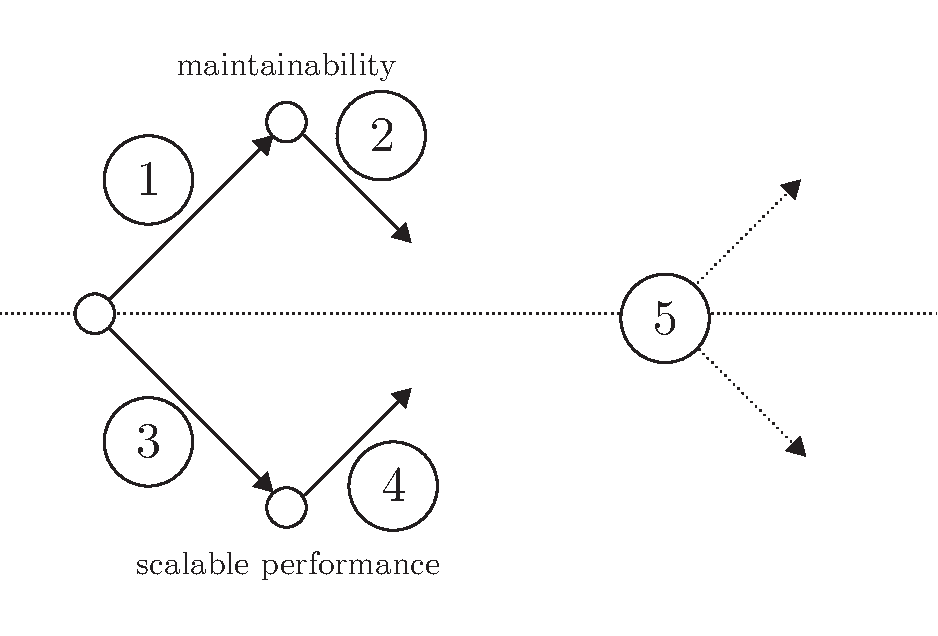
\includegraphics[width=0.6\textwidth]{../ressources/state-of-the-art.pdf}
\end{center}
\end{figure}


\subsection{Web}

Pour la justification Web, je pense que tu dois raisonner que c'est le seul marché réellement explosif, donc c'est celui que tu vises. 

Il y a pas mal d'arguments pour cibler le web :
- technologies assez peu connues, car souvent imaginées comme n'étant qu'un problème d'ihm,
- omniprésence sur internet,
- et comme tout business doit passer par Internet, il faut comprendre le web en priorité. 

Ne bloque pas trop sur le Web, pour moi c'est le contexte de fond, donc il faut que les plateformes soient orientées web. Je pense qu'un autre argument lié au web, c'est celui de TCP/IP, c'est à dire que les plateformes doivent accepter le délais dans les échanges. 
\section{From Continuations to Dues} \label{chapter5:equivalence}

This section presents the transformation from a nested imbrication of continuations into a chain of Dues.
It explains the three limitations imposed by the compiler for this transformation to preserve the semantic.
They preserve the execution order, the execution linearity and the scopes of the variables used in the operations.

\subsection{Execution order}

The compiler spots function calls with a continuation, which are similar to the abstraction in (\ref{eq:order:source}).
It wraps the function $fn$ into the function $fn_\textbf{due}$ to return a Due.
And it relocates the continuation in a call to the method $\textbf{then}$, which references the Due previously returned.
The result should be similar to (\ref{eq:order:target}).
The differences are highlighted in bold font.
\begin{equation} \label{eq:order:source}
fn([arguments], continuation)
\end{equation}
\begin{equation} \label{eq:order:target}
fn_\textbf{due}([arguments])\textbf{.then}(continuation)
\end{equation}

The execution order is different whether $continuation$ is called synchronously, or asynchronously.
If $fn$ is synchronous, it calls the $continuation$ within its execution.
It might execute $statements$ after executing $continuation$, before returning.
If $fn$ is asynchronous, the continuation is called after the end of the current execution, after $fn$.
The transformation erases this difference in the execution order.
In both cases, the transformation relocates the execution of $continuation$ after the execution of $fn$.
For synchronous $fn$, the execution order changes ; the execution of $statements$ at the end of $fn$ and the continuation switch.
The latter must be asynchronous to preserve the execution order.

\subsection{Execution linearity}

The compiler transforms a nested imbrication of continuations, which is similar to the abstraction in (\ref{eq:state:source}) into a flatten chain of calls encapsulating them, like in (\ref{eq:state:target}).
\begin{align} \label{eq:state:source}
&fn1([arguments], cont1 \{\nonumber\\
&\qquad  declare ~ variable \leftarrow result\nonumber\\
&\qquad  fn2([arguments], cont2 \{\nonumber\\
&\qquad\qquad    print ~ variable\nonumber\\
&\qquad  \})\nonumber\\
&\})
\end{align}
\begin{align} \label{eq:state:target}
&\textbf{declare variable}\nonumber\\
&fn1_\textbf{due}([arguments])\nonumber\\
&\textbf{.then}(cont1\{\nonumber\\
&\qquad  variable \leftarrow result\nonumber\\
&\qquad  fn2_\textbf{due}([arguments])\nonumber\\
&\})\nonumber\\
&\textbf{.then}(cont2\{\nonumber\\
&\qquad  print ~ variable\nonumber\\
&\})
\end{align}

An imbrication of continuations must not contain any loop, nor function definition that is not a continuation.
Both modify the linearity of the execution flow which is required for the equivalence to keep the semantic.
A call nested inside a loop returns multiple Dues, while only one is returned to continue the chain.
A function definition breaks the execution linearity.
It prevents the nested call to return the Due expected to continue the chain.
% And a call nested inside a function definition is unable to return the Due to continue the chain.
On the other hand, conditional branching leaves the execution linearity and the semantic intact.
If the nested asynchronous function is not called, the execution of the chain stops as expected.

% We demonstrate the equivalence with a sequence of two continuations.
% The equivalence is sound for a sequence of \textit{n} continuations.

\subsection{Variable scope}

In (\ref{eq:state:source}), the definitions of $cont1$ and $cont2$ are
overlapping. The $variable$ declared in $cont1$ is accessible in $cont2$ to be
printed. In (\ref{eq:state:target}), however, definitions of $cont1$ and
$cont2$ are not overlapping, they are siblings. The $variable$ is not
accessible to $cont2$. It must be relocated in a parent function to be
accessible by both $cont1$ and $cont2$. To detect such variables, the compiler
must infer their scope statically. Languages with a lexical scope define the
scope of a variable statically. Most imperative languages present a lexical
scope, like C/C++, Python, Ruby or Java. The subset of Javascript excluding
the built-in functions \texttt{with} and \texttt{eval} is also lexically
scoped. To compile Javascript, the compiler must exclude programs using these
two statements.

% # Explanation of the concept

% ## Turn-based programming.

% (see presentation on Dues)
% -> single-thread, no wait, no block and so on
% Shared heap -> no mutex, no synchronization, so it is good scalability


% Turn-based programming is an event-loop.
% It is the execution of queued events one after the other.
% An event is the association of a callback and a message.
% The callback is a small Javascript Program, designed to process the message.
% During its turn, the callback executes, and can queue events : that is register callback to be executed during a next turn.
% TODO what I mean exactly by queue events ? -> the distinction between the asynchronous operation, and the resulting event.

% ## Pipeline

% So a callback sends messages to other callbacks.
% -> It is exactly like a pipeline.
% However, all the callbacks share the same heap.
% So it is not possible to distribute the different callbacks without synchronization of this heap, or splitting the heap for each callback.
% TODO state VERY clearly this problem, it is at the core of my thesis.

% So, how to split the heap so that each callback has its own exclusive heap ?

\comment{From here, the reader should be confortable with the event-loop, and the analogy we drawn between the event-loop and a pipeline.
The problematic is now clear : how to split the heap so that each asynchronous callback has its own exclusive heap ?}

\section{Callback identification}

\subsection{\comment{TODO}}

\section{Callback isolation}

We explain in this section the compilation process we developped to isolate the memory access for each callbacks.
The result of this process should be two-fold. First each callback should have an exclusive access on a region of the memory. So that two different callback can be executed in parallel. And it should be clear for each callback, what are the variable needed from upstream callbacks, and what are the variable to send downstream.

\subsection{Propagation of variables}


\subsubsection{Scope identification}

In section \ref{??? Javascript scope / closure}, we explained that Javascript is roughly lexically scoped.
A consequence is that the declaration of contexts can be inferred statically.
For example, in a lexically scoped, strongly typed, compiled language, the compiler know the content of each scope during compile time, and can prepare the memory stack to store the variables in each scope.

In most languages, the memory is in two parts : the stack, and the heap.
The stack is statically scoped, and its layout is known at compile time.
The heap, on the other hand is dynamically allocated. Its layout is built at run time.

But Javascript is a dynamic language, perhaps the most dynamic of all languages.
It doesn't have this distinction between stack and heap. Every variable is dynamically allocated on the heap.
That induce two consequences.
The first is that Javascript provides two statements to dynamically modify the lexial scope : \texttt{eval} and \texttt{with}.
The second is that to know the layout of the heap, we need to use static analysis tools.
In the next two sections, we adress these two consequences.

\subsubsection{Break the lexical scope} \label{???:breakscope}

Without these statements, \texttt{eval} and \texttt{with}, Javascript is lexically scoped. It is possible to infer the scope of each variable at compile time.


The \texttt{with} statement continue the execution using an expression as the lexical scope.
As the provided expression is dynamically evaluated, it is possible to dynamically modify the lexical scope.
The code snippet below show an example of such a situation.

\begin{code}
var aliveCat = {isAlive: true};
var deadCat = {isDead: true}

with (Math.random() > 0.5 ? aliveCat : deadCat) {
  isAlive;
  // Half the time -> ReferenceError: isAlive is not defined
  // Half the time -> true;
}
\end{code}

The variable \texttt{isAlive} is defined only in the object \texttt{aliveCat}.
The presence of the variable \texttt{isAlive} in the lexical environment within the \texttt{with} statement cannot be determined statically, as the lexical environment is dynamically linked to either \texttt{aliveCat} or \texttt{deadCat}.

Note that the MDN reference page on \texttt{with}\ftnt{https://developer.mozilla.org/en-US/docs/Web/JavaScript/Reference/Statements/with} says that \textit{Using \texttt{with} is not recommended, and is forbidden in ECMAScript 5 strict mode.}

The \texttt{}

% TODO and specify that Javascript is roughly lexically scoped : it is not completely lexically scoped, and five examples to backup that.

Not to be mistaken with the \texttt{this} operator.
It is possible to dynamically change the content of an object,  
% TODO continue this paragraph about how the this operator change the properties of an object. 
% Does it change the lexical scope, if that object is actually used as a context elsewhere ? -> No, I don't think so.
% But ask on SO, just to be sure.

\begin{code}
function stuff() {
  this.x = 42;
}

stuff.call({})

\end{code}

% Javascript is lexically scoped, therefore we can identify the the scope of variable statically.
% (At the exception of eval and with : with is forbidden from strict mode, so that is not a bigdeal, howether, eval is sometimes used in smart ways, but most of the time it is monomorphic (I don't exactly know what that means, I heard from Floreat, it must be something related to PL community)).

% The compiler identifies the variables shared by multiple callbacks from their scope.
% TODO explain this in depth.
% Function scope, closures, and so on ...



However, even if Javascript is lexically scoped, the memory is still dynamicall allocated and manipualeted, so that it is not possible to actually infer the memory layout at compiler time only with lexical scope analysis, and without deeper static analysis.

\subsubsection{Scope Leaking}

% Javascript uses a pass-by-sharing paradigm.
% That means that sometimes the argument of a call are passed by value, sometimes by reference (atomic data type (number, string, bool) -> by value, complex data type (objects) -> by reference).
% That means that the modification of a local variable can affect variable in seemingly unrelated scopes.
% It seems that the points-to analysis is what is used to find stuffs like that (side-effects ?).

% TODO what we are talking about here are aliases.

% TODO I am stating here that in low-level language, the memory access is so fine, that it is difficult to exactly pin down the memory layout in term of object, it is rather seen as a big array of memory adresses.
% While in higher-level language, like Javascript, the memory access is at the property level (it is not possible to access memory down to the adress), so it could be easier (maybe, just not harder) to infer the dynamic memory layout from source.
To infer the layout of the heap at compile time, static analysis tools are used, like the points-to analysis, developped by Andersen in its PhD thesis \cite{Andersen1994}.
For such analysis, the memory is splitted at the access scale.
In low-level languages, like C/C++, the memory is mainly managed by the developer. Allowing access to the memory at a small grained scale : up to the address.
It impose the analysis to split the memory to the adress scale in some cases.
% TODO Backup that, HEAVILY
In higher-level languages, like Javascript, the developer cannot access the memory to the adress scale.
The memory is accessed at a coarser scale : the property scale.
(At the exception of some arrays and buffers, that mimic, and are mapped to actual memory adresses for performance reasons.)
% TODO find exactly the references for these buffers : I think of ArrayBuffer, and sharedArray ... but I am not sure. Need more inspection.

\subsubsection{Propagation of execution and variables}

For the execution of each callback / stage, the corresponding part of the state is local, and the rest is remote, and inaccessible.
We are going to explain why it must remain inaccessible.

While a callback is executing a request, the previous callback (the up stream callback) is executing the next request.
The next request will arrive at the current callback some time in the future.
The modification done in the state of the upstream callback will propagate only later in the current callback.
The state of the upstream callback is in a different time frame than the state of the current callback.

To really understand that, we need to compare this execution with the execution on a unique event-loop.
If the current callback executes, then the upstream callback might have, or might not have started to execute the next request.
But as soon as the current callback executes, the modifications done on the states, are immediatly propagated, so that the upstream callback can take them into account for the next request.

However, if the two callbacks are distant, then the modification of the current callback will not immediatly propagate to the upstream callback.
During the propagation, the upstream callback might execute requests than would not be aware of the state modification from the current callback (from downstream).
That is why we say the upstream callback and the current callback are in two different time frame.
Propagating the state modification upstream is like going backward in time, it is impossible.
That is why the execution, and the state modification propagation must always flow downstream.

As a note, I must add that if an upstream and a downstream callbacks are on the same event-loop, then this doesn't apply. it is like a loop in the time : the modification immediatly propagate from downstream to upstream.






% The execution progress downstream, following the message stream.
% TODO state very clearly this proposition, it is the second core of my thesis (and I love the idea, it relates directly to reality, graivity, and the fabric of the universe <3).

% Because the propagation of the modification is not instantaneous, going back upstream is like going backward in time : it is impossible.
% Therefore, a variable cannot be read upstream a write.
% And it cannot be write downstream either.

% In other words, only one callback can write on a variable -> seems obvious from previous sections.


% In promises, because the heap is not shared, things are less restrictive.
% Multiple stages can read and write the same variable, because the propagation of modification is instantaneous, due to the shared heap.





% TODO write about what it implies to detect continuation in variable, or other expressions.

% Why can we only detect continuations declared in situ.
% If a continuation is passed as a variable, we don't know for sure what is the function associated with, and the closure of that function.

\subsection{Real test case} \label{chapter5:flx:evaluation}

The compiler is tested on a real application, gifsockets-server\ftnt{https://github.com/twolfson/gifsockets-server}.
This test proves the possibility for an application to be compiled into a network of independent parts.
It shows the current limitations of this isolation and the modifications needed on the application to circumvent them.

\begin{code}[js, caption={Simplified version of gifsockets-server},label={lst:gifsocket}]
var express = require('express'),
    app = express(),
    routes = require('gifsockets-middleware'), //@\label{lst:gifsocket:gif-mw}@
    getRawBody = require('raw-body');

function bodyParser(limit) { //@\label{lst:gifsocket:bodyParser}@
  return function saveBody(req, res, next) { //@\label{lst:gifsocket:saveBody}@
    getRawBody(req, { //@\label{lst:gifsocket:getRawBody}@
      expected: req.headers['content-length'],
      limit: limit
    }, function (err, buffer) { //@\label{lst:gifsocket:callback}@
      req.body = buffer;
      next(); //@\label{lst:gifsocket:next}@
    });
  };
}

app.post('/image/text', bodyParser(1 * 1024 * 1024), routes.writeTextToImages); //@\label{lst:gifsocket:app.post}@
app.listen(8000);
\end{code}

This application, simplified in listing \ref{lst:gifsocket}, is a real-time chat using gif-based communication channels.
It was selected from the evaluation set of the Due compiler because it is simple enough to illustrate this evaluation.
% \cite{Brodu2015}
%  from the \texttt{npm} registry because it depends on \texttt{express}, it is tested, working, and simple enough to illustrate this evaluation.
The server transforms the received text into a gif frame, and pushes it back to a never-ending gif to be displayed on the client.

On line \ref{lst:gifsocket:app.post}, the application registers two functions to process the requests received on the url \texttt{/image/text}.
The closure \texttt{saveBody}, line \ref{lst:gifsocket:saveBody}, returned by \texttt{bodyParser}, line \ref{lst:gifsocket:bodyParser}, and the method \texttt{routes.write\-Text\-To\-Images} from the external module \texttt{gifsockets-\-middleware}, line \ref{lst:gifsocket:gif-mw}.
The closure \texttt{saveBody} calls the asynchronous function \texttt{getRawBody} to get the request body.
Its callback handles the errors, and calls \texttt{next} to continue processing the request with the next function, \texttt{routes.write\-Text\-To\-Images}.

\subsubsection{Compilation} \label{chapter5:flx:evaluation:compilation}

% We compile this application with the compiler
The compilation result is in listing \ref{lst:flx-gifsocket}.
The function call \texttt{app.post}, line \ref{lst:gifsocket:app.post}, is a rupture point.
However, its callbacks, \texttt{bodyParser} and \texttt{routes.write\-Text\-To\-Images} are not declared \textit{in situ}.
They are evaluated as functions only at runtime.
As precised previously, the compiler discards these callbacks to avoid altering the semantic. % by moving or modifying their definition.
% For this reason, the compiler ignores this rupture point, to avoid interfering with the evaluation.

\begin{code}[flx, caption={Compilation result of gifsockets-server},label={lst:flx-gifsocket}]
flx main & express {req}
>> anonymous_1000 [req, next]
  var express = require('express'),
      app = express(),
      routes = require('gifsockets-middleware'), //@\label{lst:flx-gifsocket:gif-mw}@
      getRawBody = require('raw-body');

  function bodyParser(limit) { //@\label{lst:flx-gifsocket:bodyParser}@
    return function saveBody(req, res, next) { //@\label{lst:flx-gifsocket:saveBody}@
      getRawBody(req, { //@\label{lst:flx-gifsocket:getRawBody}@
        expected: req.headers['content-length'], //@\label{lst:flx-gifsocket:req.headers}@
        limit: limit
      }, >> anonymous_1000 [req, next]);
    };
  }

  app.post('/image/text', bodyParser(1 * 1024 * 1024), routes.writeTextToImages); //@\label{lst:flx-gifsocket:app.post}@
  app.listen(8000);

flx anonymous_1000
-> null
  function (err, buffer) { //@\label{lst:flx-gifsocket:callback}@
    req.body = buffer; //@\label{lst:flx-gifsocket:buffer}@
    next(); //@\label{lst:flx-gifsocket:next}@
  }
\end{code}

The compiler detects a rupture point : the function \texttt{get\-Raw\-Body} and its anonymous callback, line \ref{lst:gifsocket:callback}.
It encapsulates this callback in a fluxion named \texttt{anony\-mous\_\-1000}.
The callback is replaced with a stream placeholder to send the message stream to this downstream fluxion.
The variables \texttt{req} and \texttt{next} are appended to this message stream, to propagate their value from the \texttt{main} fluxion to the \texttt{anony\-mous\_\-1000} fluxion.

When \texttt{anony\-mous\_\-1000} is not isolated from the \texttt{main} fluxion, as if they belong to the same group, the compilation result works as expected.
The variables used in the fluxion, \texttt{req} and \texttt{next}, are still shared between the two fluxions.
In this situation fluxions are quite similar to Dues regarding memory shareing.
Our goal is to isolate the two fluxions, to be able to safely parallelize their executions.

\subsubsection{Isolation} \label{chapter5:flx:evaluation:isolation}

In listing \ref{lst:flx-gifsocket}, the fluxion \texttt{anony\-mous\_\-1000} modifies the object \texttt{req}, line \ref{lst:flx-gifsocket:buffer}, to store the text of the received request, and it calls \texttt{next} to continue the execution, line \ref{lst:flx-gifsocket:next}.
\texttt{req} is an alias to a memory location used in multiple palces in code.
Therefore, these operations produce side-effects that should propagate in the whole application, but the isolation prevents this propagation.
Isolating the fluxion \texttt{anony\-mous\_\-1000} produces runtime exceptions.
The next paragraph details how this situation is handled to allow the application to be parallelized.

\paragraph{Variable \texttt{req}}

The variable \texttt{req} is read in fluxion \texttt{main}, lines \ref{lst:flx-gifsocket:getRawBody} and \ref{lst:flx-gifsocket:req.headers}.
Then its property \texttt{body} is associated to \texttt{buffer} in fluxion \texttt{anony\-mous\_\-1000}, line \ref{lst:flx-gifsocket:buffer}.
The compiler is unable to identify the aliases of this variable. % further usages.
However, the side effect resulting from this association impacts a variable in the scope of the next callback, \texttt{routes.write\-Text\-To\-Images}.
In this test case, the application is modified manually to explicitly propagate this side-effect to the next callback through the function \texttt{next}.
The modifications of this function are explained further in the next paragraph.

\paragraph{Closure \texttt{next}}

The function \texttt{next} is a closure provided by the \texttt{express} \texttt{Router} to continue the execution with the next function to handle the client request.
Because it indirectly relies on the variable \texttt{req}, it is impossible to isolate its execution with the \texttt{anony\-mous\_\-1000} fluxion.
Instead, we modify \texttt{express}, so as to be compatible with the fluxional execution model.
We explain the modifications below.

\begin{code}[flx, caption={Simplified modification on the compiled result},label={lst:mflx-gifsocket}]
flx anonymous_1000
-> express_dispatcher
  function (err, buffer) { //@\label{lst:mflx-gifsocket:callback}@
    req.body = buffer; //@\label{lst:mflx-gifsocket:buffer}@
    next_placeholder(req, -> express_dispatcher); //@\label{lst:mflx-gifsocket:next-placeholder}@
  }

flx express_dispatcher & express {req} //@\label{lst:mflx-gifsocket:express-dispatcher}@
-> null
  function (modified_req) {
    merge(req, modified_req);
    next(); //@\label{lst:mflx-gifsocket:next}@
  }
\end{code}

In listing \ref{lst:gifsocket}, the function \texttt{next} is a continuation allowing the anonymous callback, line \ref{lst:gifsocket:callback}, to call the next function to handle the request.
To isolate the anonymous callback into \texttt{anonymous\_\-1000}, \texttt{next} is replaced by a rupture point.
This replacement is illustrated in listing \ref{lst:mflx-gifsocket}.
The \texttt{express} \texttt{Router} registers a fluxion named \texttt{express\_\-dispatcher}, line \ref{lst:mflx-gifsocket:express-dispatcher}, to continue the execution after the fluxion \texttt{anony\-mous\_\-1000}.
This fluxion is in the same group \texttt{express} as the \texttt{main} fluxion, hence it has access to the original variable \texttt{req}, and to the original function \texttt{next}.
The call to the original \texttt{next} function is replaced by a placeholder to push the stream to the fluxion \texttt{express\_\-dispatcher}, line \ref{lst:mflx-gifsocket:next-placeholder}.
The fluxion \texttt{express\_\-dispatcher} receives the stream from the upstream fluxion \texttt{anony\-mous\_\-1000}, merges back the modification in the variable \texttt{req} to propagate the side effects, and finally calls the original function \texttt{next} to continue the execution, line \ref{lst:mflx-gifsocket:next}.

After the modifications detailed above, the server works as expected.
The isolated fluxion correctly receives, and returns its serialized messages.
The client successfully receives a gif frame containing the text.



\subsection{Limitations}

The static analysis used for this compiler presents some limitations.
It is unable to analyze code with dynamic behaviors.
Higher-order programming leads to more productivity partly beacuse it rely on such dynamic behavior to extend expressivity.
Precisely, it allows more levels of indirections.

\subsubsection{Levels of Indirections}

The indirection is an abstraction between the value, and its manipulation.
In listing \ref{lst:indirection}, the variables \texttt{a} and \texttt{b} point both to the same memory object.
The function \texttt{fn} introduces a level of indirection between the real object \texttt{a} and its manipulation handle, \texttt{b};
% Actually, the variable \texttt{a} already introduces a level of indirection between the real object and the handle \texttt{a}.

\begin{code}[js,
  caption={One level of Indirection},
  label={lst:indirection}]
var a = {
      // an object;
    };

fn(b) {
  // modify b;
}

fn(a);
\end{code}

\subsubsection{Uncertainties}

The indirection is trivial to resolve in listing \ref{lst:indirection}.
It only needs to have access to the definition of \texttt{a} and of \texttt{fn}.
%A very simple static analysis could resolve it.
However, in listing \ref{lst:indirections}, the array \texttt{handlers} introduces a new level of indirection.
The static analysis now needs to have access to the definition of \texttt{i} and of the \texttt{handlers}.
If this definition is provided by an external input, it is not available statically, hence, it adds an uncertainty during the analysis. 

\begin{code}[js,
  caption={Two levels of indirection},
  label={lst:indirections}]
var a = {
      // an object;
    },
    handlers = [
      // definition of fn handlers;
    ],
    i = ?;

handlers[i](a);
handlers[i+1](a);
\end{code}

These examples are extremely simplified.
A real application contains enough indirections for the static analysis to be overwhelmed by uncertainties, and to be unable to resolve the variables.
If a variable is left unresolved, it is impossible to assure its scope and its aliases.
Therefore, the compiler is unable to isolate it into a fluxion, or to distribute its modification by messages.

Moreover, it leads the compiler to ignore the rupture points not defined \textit{in situ}, because their modifications could impact the semantic.
The reason for this precaution, is that the compiler is unable to assure where the function is used, and the scope of its variables.
Therefore, it is unable to assure that the modification will conserve the semantic.

\subsubsection{Dynamic Resolution}

In a web application, this variable \texttt{i} might be part of the user request, which is available only at runtime.
It eventually introduces an uncertainty.

This dynamic resolution of variables is precisely what increase expressiveness.
Trying to resolve them statically is equivalent to restrict expressiveness.
No static analysis can overstep these limitations.
Only a dynamic analysis could analysis the resolved indirections during run time to overstep these limitations correctly.


